%!TEX root = ../../main.tex
\frame{
\subsection{3D-Deskriptor}
\frametitle{3D-Deskriptor?}
	\setbeamertemplate{description item}[align left]
	\begin{description}
		\item[Eingabe] Tiefeninformationsgewinnug $\rightarrow$ \textbf{3D-Punktwolke}
		\item[Verarbeitung] Berechnung, welche Punkt und seine Nachbarschaft betrachtet.
		\item[Ausgabe] Möglichst eindeutige Beschreibung
	\end{description}

	    \begin{figure}
        \centering
        \begin{subfigure}[b]{0.3\textwidth}
            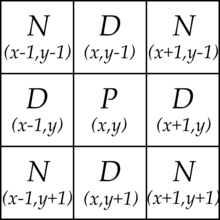
\includegraphics[width=\textwidth]{topics/intro/n2d.png}
            \caption{2D-Nachbarschaft}
            \label{fig:2dn}
        \end{subfigure}
        ~~~
        \begin{subfigure}[b]{0.3\textwidth}
            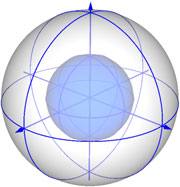
\includegraphics[width=\textwidth]{topics/intro/n3d.png}
            \caption{3D-Nachbarschaft}
            \label{fig:3dn}
        \end{subfigure}
    \end{figure}


}

\subsection{Objekterkennung}
\frame{
	\frametitle{Objekterkennung}
	Finde bekanntes Objekt in einer Szene:
	\begin{enumerate}
		\item Berechne Deskriptoren für Modell
		\item Berechne Deskriptoren für Szene
		\item Vergleiche berechnete Deskriptoren
	\end{enumerate}


		 \begin{figure}
        \centering
        \begin{subfigure}[b]{0.45\textwidth}
            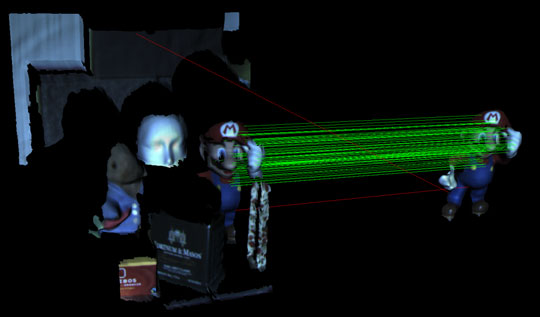
\includegraphics[width=\textwidth]{topics/intro/matchingScene.png}
            \caption{Finde Objekt}
            \label{fig:find}
        \end{subfigure}
        ~~~
        \begin{subfigure}[b]{0.45\textwidth}
           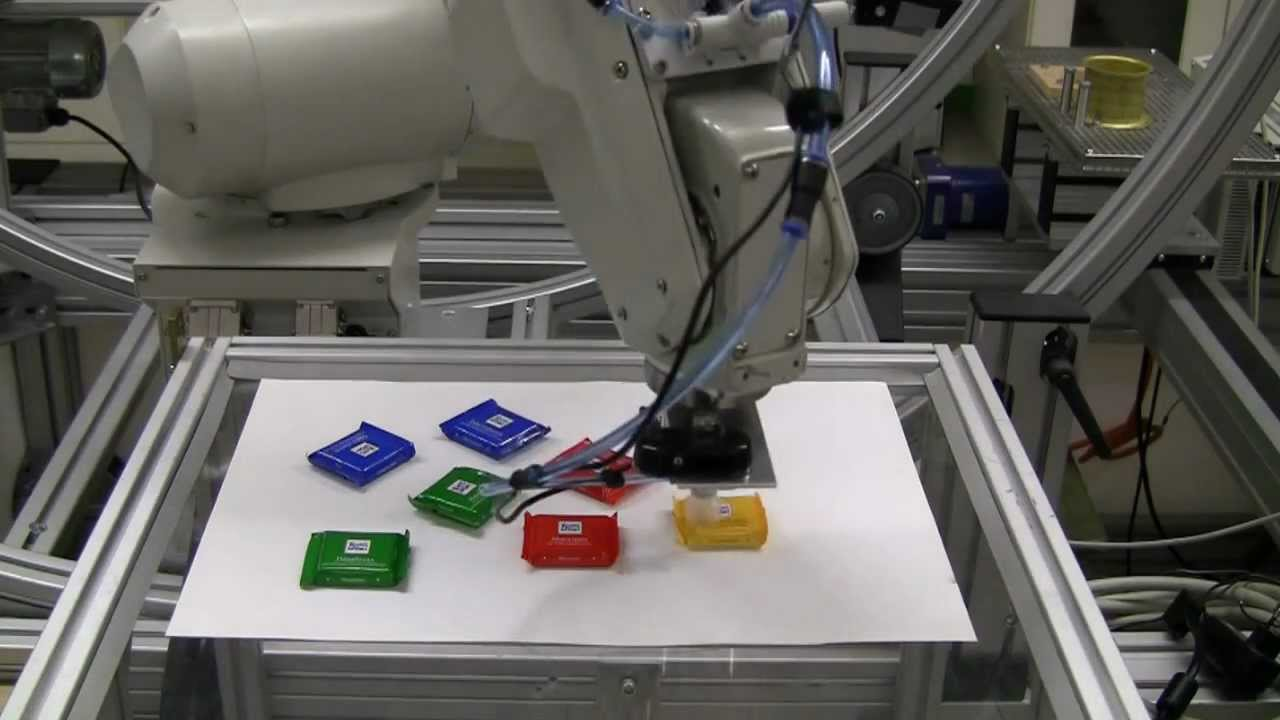
\includegraphics[width=\textwidth]{topics/intro/objRec1.jpg}
            \caption{Bestimme Lage.}
            \label{fig:3dn}
        \end{subfigure}
    \end{figure}

	\centering
		
}

\subsection{Rekonstruktion}
\frame{
	\frametitle{Rekonstruktion}

\begin{flushleft}
\setbeamertemplate{description item}[align left]
            \begin{description}
            	\item[Genauigkeit] von verwendeten Verfahren nicht ausreichend.
            	\item[Textur] ist von entscheidender Bedeutung
            	\item[Interpolation] von gewonnenen Bildpunkten.
            	\item[Besseres] Modell der Umgebung
			\end{description}

		\begin{itemize}
			\item Automatisierte Baumaschinen
			\item Automatische Landung von Raumsonden
		\end{itemize}
\end{flushleft}

\setbeamertemplate{description item}[align left]
            \begin{description}
            	\item[Daten] von mehreren Sensoren/Verfahren.
            	\item[Kombination] zu einer einzigen Punktwolke
			\end{description}

}